\documentclass[tikz]{standalone}
\newcommand{\printSQ}[3]{\filldraw [fill=#3, draw=black] (#1-0.5,#2-0.5) rectangle (#1+0.5,#2+0.5);}
\begin{document}
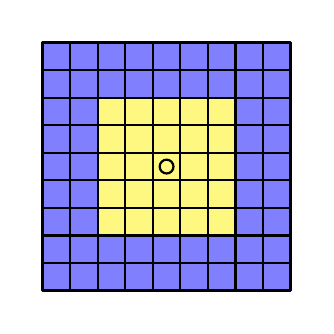
\begin{tikzpicture}[thick,scale=0.35,line join=round,>=latex]
  \foreach \i in {-4,...,4} {
      \foreach \j in {-4,...,4} {
          \printSQ{\i}{\j}{blue!50}
        }
    }
  
  \foreach \i in {-2,...,2} {
      \foreach \j in {-2,...,2} {
          \printSQ{\i}{\j}{yellow!50}
        }
    }
  
  \draw (0,0) circle (0.25);
  \draw [white] (-5,-5) rectangle (5,5);
\end{tikzpicture}
\end{document}